\documentclass[border=10pt]{standalone} 
%%%<
\usepackage{verbatim}
%%%>
\begin{comment}
:Title: Decision tree
:Tags: Trees;Graphics;TikZ
:Author: Stefan Kottwitz
:Slug: decision-tree

A horizontal tree, growing to the right.
I created a basic style for tree nodes, and
derived styles for specific kinds of nodes.

Full explanation in Chapter 9, Creating Graphics:
[Growing a tree](https://latex-cookbook.net/tree/)
\end{comment}
\usepackage{tikz}
\tikzset{
  treenode/.style = {shape=rectangle, rounded corners,
                     draw, align=center,
                     top color=white, bottom color=blue!10},
  treenodeD/.style = {shape=circle,
                     draw, align=center,
                     top color=white, bottom color=blue!10},
  root/.style     = {treenode, bottom color=red!15},,
  env/.style      = {treenode, font=\ttfamily\normalsize},
  dummy/.style    = {circle,draw}
}
\begin{document}
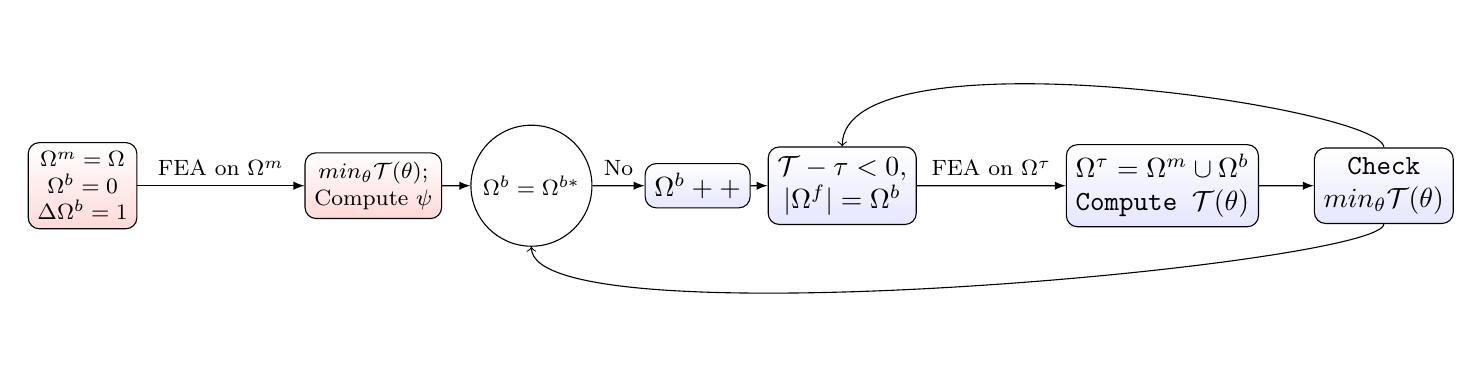
\begin{tikzpicture}
  [
    grow                    = right,
    sibling distance        = 5em,
    level distance          = 8em,
    edge from parent/.style = {draw, -latex},
    every node/.style       = {font=\footnotesize},
    sloped
  ]
  \node [root] (P){$\Omega^{m}=\Omega$\\$\Omega^{b}=0$ \\ $\Delta\Omega^{b}=1$}
    child { node [root, right=0.2] (A) {$min_{\theta}\mathcal{T}(\theta)$; \\ Compute $\psi$}
      child { node [dummy, left =0.8] (B) {$\Omega^{b}=\Omega^{b*}$}
        child { node [env, left =0.8] (C) {$\Omega^{b}++$}
            child{ node [env, left =0.8] (D) {$\mathcal{T}-\tau <0,$\\$|\Omega^{f}|=\Omega^{b}$}
                child{ node [env, right =0.8] (E) {$\Omega^{\tau}=\Omega^{m}\cup\Omega^{b}$\\
                Compute $\mathcal{T}(\theta)$}
                    child{ node [env] (F) {Check \\ $min_{\theta}\mathcal{T}(\theta)$} }
                    edge from parent node [above]{FEA on $\Omega^{\tau}$}}}
                edge from parent node [above] {No}}}
            edge from parent node [above] {FEA on $\Omega^{m}$} };
\draw[->] (F)..controls +(south:1) and +(south:2)..(B);
\draw[->] (F)..controls +(north:1) and +(north:2)..(D);
\end{tikzpicture}
\end{document}